\chapter{Wykorzystane technologie}

\section{Spis użytych technologii}
System został napisany jako aplikacja webowa, w~języku Java, w~wersji 1.8. Java to obiektowy, silnie typowany, wieloplatformowy język programowania, obecnie rozwijany przez firmę Oracle Corporation. Ponadto do realizacji systemu wykorzystano takie istniejące rozwiązania jak:

\begin{itemize}

\item Git - rozproszony system kontroli wersji (ang. version control system). System kontroli wersji pozwala śledzić zmiany w~dokumencie. Zapisuje on kto, kiedy i~jakie modyfikacje w~dokumencie dokonał. Programowanie jest dziedziną, gdzie systemy kontroli wersji wykorzystuje się powszechnie. Ułatwiają one pracę wielu osób nad jednym dokumentem, wycofywanie nieprawidłowych zmian, znalezienie winnego błędnej modyfikacji, czy proces przeglądu kodu \cite{PoCoKontrola}. W~programowaniu Git to jeden z~obecnie (2014) najpopularniejszych systemów kontroli wersji, zyskuje on na znaczeniu w~ostatnich latach (2011-2014) \cite{EclipseSurvey};

\medskip
\item GitHub - usługa internetowa, pozwalająca na przechowywanie repozytoriów Git. Oferuje całą bazową funkcjonalność systemu Git, a~także ją dodatkowo ją rozszerza. Z~usługi tej korzysta obecnie 12,4 mln osób, którzy rozwijają projekty w~ramach 31,7 mln repozytoriów systemu kontroli wersji \cite{GitHubPress}. Darmowe konto pozwala przechowywać nieograniczoną liczbę repozytoriów publicznych, do których można zaprosić nieograniczoną liczbę współautorów. Za możliwość utworzenia repozytorium prywatnego trzeba zapłacić;

\medskip
\item Gradle - system zarządzania zależnościami dla języka Java. Gradle jest alternatywną dla znacznie popularniejszych systemów takich jak Maven, czy Ant \cite{EclipseSurvey}. Autor dokonał wyboru systemu zarządzania zależnościami pomiędzy systemami Maven i~Gradle - systemy te są wspierane przez wybraną bazową platformę programistyczną (Spring Framework). Ostateczny wybór jest kwestią indywidualnych upodobań autora. Autor uważa, że składnia używana przez Gradle jest znacznie czytelniejsza niż w~Maven - w~szczególności lista zależności. System zarządzania zależnościami odpowiada za proces budowania do wybranego wspieranego formatu wynikowego, a~także za pobranie pakietów (plików .jar) zależności przed procesem budowania oprogramowania. Dzięki temu nie ma potrzeby dostarczania z~kodem źródłowym systemu także pakietów zależności - te zostaną pobrane automatycznie. System zarządzania zależnościami, we współpracy ze zintegrowanym środowiskiem programistycznym (ang. Integrated Development Environment, IDE), potrafi także pobierać dokumentacje i~kody źródłowe wykorzystywanych zależności - co znacząco podnosi komfort programowania;

\medskip
\item Spring Framework - platforma programistyczna (ang. framework) dla języka Java, dostarcza takie komponenty jak: szkielet wzorca architektonicznego Model-Widok-Kontroler (ang. Model-view-constoller, MVC), mechanizm wstrzykiwanie zależności, mechanizm zarządzania transakcjami, mechanizm zarządzania dostępem do danych i~inne. Platforma ta jest podstawą systemu. Definiuje ona główną architekturę systemu. Zastosowanie platformy z~reguły poprawia jakość pisanego kodu, podnosi efektywność procesu programowania, a~także zwiększa niezawodność systemu \cite{Framework}. W~zamian podnosi złożoność systemu, oraz może obniżyć jego wydajność \cite{Framework};

\medskip
\item Spring Boot - biblioteka dostarczająca strategię \textquote{konwencja, nie konfiguracja} (ang.~convention over configuration) dla platformy Spring. Jest to dodatkowa warstwa, która wykorzystuje jako zależność oryginalną platformę Spring Framework. Jej celem jest minimalizacja liczby konfiguracji wymaganej do uruchomienia strony internetowej z~wykorzystaniem platformy Spring. Biblioteka ta została wydana w~kwietniu 2014 roku, jako \textquote{recepta} na zbytnie skomplikowanie bazowej platformy Spring Framework, która wymaga dużej liczby konfiguracji~i szerokiej wiedzy na temat sposobu jej działania \cite{SpringIssueBoot}. Oficjalnym \textquote{zalążkiem} tej biblioteki jest zgłoszenie, w~systemie zgłaszania i~śledzenia błędów (ang. issue tracker) platformy Spring Framework,~w 2012 roku propozycji \textquote{improve support for 'containerless' web application architectures}, gdzie Mike Youngstrom opisał wady istniejącego rozwiązania i~zaproponował zmianę koncepcji \cite{SpringIssueBoot};

\medskip
\item Jetty - serwer stron internetowych i~serwletów języka Java, napisany w~całości w~tym języku. Może działać w~trybie wbudowanym (ang. embedded mode). Jeden z~dwóch, obok Tomcat, serwerów wspieranych przez Spring Boot. Autor wybrał ten serwer na podstawie własnych preferencji, kierując się głównie historią wersji obydwu serwerów, która wskazuje iż rozwój Jetty jest aktywniejszy, i szybciej podąża za nowymi technologiami;

\medskip
\item H2 - system zarządzania relacyjną bazą danych (ang. relational database management system, RDBMS). Jest napisany w~języku Java, wspiera standard SQL, charakteryzuje go wysoka wydajność w~trybie wbudowanym i~obsługa transakcji bazodanowych \cite{H2Performance}. Autor w~ramach pracy zdecydował się użyć bazy danych w~trybie wbudowanym. Pod względem wydajności wybrana baza z~sukcesem konkuruje z~konkurencją, także tą, która wymaga do działania serwera, tzn. działających w~trybie klient-serwer (ang.~client-server mode) \cite{H2Performance}. Autor nie rozważał możliwości użycia baz nierelacyjnych (typu NoSQL), ani baz obiektowych (ang. object database);

\medskip
\item Hibernate ORM - biblioteka dla języka Java dostarczająca mechanizm mapowania z~relacyjnego systemu bazodanowego na obiekty w~języku Java. Implementuje ona oficjalny standard mapowania relacyjno-obiektowego (ang. object-Relational Mapping, ORM) dla języka Java: Java Persistence API (JPA). Mechanizm mapowania relacyjno-obiektowego pozwala odwoływać się do danych, zapisanych w~bazie w~sposób relacyjny, w~sposób obiektowy z~poziomu języka programowania. Klasa reprezentująca tabelę w~bazie danych nazwa się encja (ang. entity). Za operację typu CRUD (ang. create, read, update, delete; pol. utwórz, odczytaj, aktualizuj, usuń) na warswie bazy danych odpowiada menadżer encji (ang. entity manager). Wykorzystanie ORM odciąża programistę od potrzeby pisania zapytań SQL (operowanie na encjach jest także bardziej naturalne dla programowania obiektowego), oraz zabezpiecza przed atakami typu \textquote{SQL injection};

\medskip
\item Thymeleaf - biblioteka dla języka Java dostarczająca silnik szablonów do przetwarzania i~generowania dokumentów HTML, XML, plików JavaScript, CSS. Pisany system jest dynamiczny. Informacje wyświetlane użytkownikowi zależą od aktualnego stanu systemu. Wykorzystanie silnika szablonów zapewnia wydzielenie warstwy widoku, zgodnie z~wykorzystanym wzorem model-widok-kontroler. Widok zawiera referencję do modelu, otrzymaną od kontrolera skąd może pobrać za każdym razem aktualne dane. Wybrany silnik szablonów posiada wsparcie dla najnowszej wersji standardu HTML (HTML5), internacjonalizacji oraz automatycznie kontroluje poprawność składniową generowanego dokumentu;

\medskip
\item OAuth2 - otwarty standard autoryzacji użytkowników. Określa on przebieg procesu dostępu do zasobów aplikacji trzeciej, bez udostępniania danych autoryzujących. Użytkownik w~systemie musi być autoryzowany. Ustalonym sposobem autoryzacji jest OAuth2, gdyż to właśnie ten sposób jest wpierany przez usługę GitHub;

\medskip
\item pac4j: Spring Web MVC / Spring Boot - biblioteka dla języka Java dostarczająca mechanizmy pozwalające zabezpieczyć systemy webowe przed dostępem osób nieautoryzowanych. Budowa tego mechanizmu jest modułowa. Dołączając odpowiedni można przy jej użyciu zrealizować właściwie każdy sposób uwierzytelnienia (ang. authentication) i~autoryzacji (ang. authorization) użytkownika;

\medskip
\item pac4j-oauth: moduł biblioteki pac4j pozwalający zrealizować system autoryzacji z~użyciem standardu OAuth2. W~projektowanej aplikacji rolę serwera autoryzacji (ang. authorization server) i~serwera zasobów (ang. resource server) pełni usługa GitHub;

\medskip
\item GitHub API v3 (GitHub API) - interfejs programistyczny pozwalający w~sposób programowy komunikować się z~usługą GitHub w~celu uzyskania lub modyfikacji zasobów, które one przechowuje. Interfejs programistyczny udostępniony przez GitHub jest bardzo zaawansowany. Można przy jego użyciu wykonać właściwie wszystkie akcje dostępne w~serwisie, w~tym te najbardziej interesujące w~kontekście budowanego systemu: odczyt podstawowych informacji na temat repozytorium (lista powieleń, lista gałęzi, nazwa gałęzi głównej, adres do pobrania repozytorium, możliwość utworzenia nowego);

\medskip
\item com.squareup: OkHttp - biblioteka dla języka Java, implementacja klienta http z~możliwością zapamiętywania odpowiedzi w~pamięci podręcznej (ang. cache);

\medskip
\item org.kohsuke: github-api - biblioteka dla języka Java będąca implementacją komunikacji z~GitHub API w~tym języku. Udostępniona dokumentacja API opisuje istniejące zasoby i~sposoby odwołania do nich. Nie istnieje jednak oficjalna implementacja dostępu do wspominanego API w~jakimś konkretnym języku programowania. Wybrana biblioteka udostępnia obiektowo-zorientowaną reprezentację komunikacji ze wspominanym API. Autor biblioteki deklaruje iż pokrywa ona \textquote{znaczną część} API. Autor sprawdził, iż pokrycie jest wystarczające do zrealizowana systemu;

\medskip
\item Eclipse JGit - biblioteka dla języka Java pozwalająca zarządzać repozytorium Git programowo, z~poziomu tego języka. W~opinii autora akcje takiej jak: zatwierdzanie zmian, synchronizacja repozytorium lokalnego ze zdalnym za pomocą GitHub API są mało intuicyjne i~stosunkowo trudne. Autor zdecydował się użyć innej biblioteki do tych zadań. Wybrana biblioteka JGit realizuje te zadania wykorzystując system plików - działa podobnie jak program \textquote{git}. Jest to biblioteka generyczna - znajduje zastosowanie zarówno dla repozytoriów lokalnych, jak i~dla~dowolnej usługi przechowującej repozytorium Git zdalnie;

\medskip
\item Apache POI - biblioteka dla języka Java, umożliwia generowanie dokumentów pakietu Microsoft Office (w~tym arkuszy Excel) programowo, z~poziomu tego języka. Podsumowania przeglądów system generuje jako arkusz MS Excel. Zastosowana biblioteka potrafi generować zarówno starsze pliki pakietu Office (przed wersją 2007), jak i~nowsze (od wersji 2007, z~dodatkową literą \textquote{x} w~rozszerzeniu);

\end{itemize}

\section{Wielokrotne użycie}
Wymyślanie koła na nowo nie zawsze jest dobrym rozwiązaniem. Pisaniu aplikacji sprzyjała idea wielokrotnego użycia. Wykorzystano jak najwięcej istniejących rozwiązań, w~większości znanych i~dojrzałych. Istotnym założeniem projektowania była integracja z~istniejącymi i~powszechnie wykorzystanymi usługami.
 
\subsection{Git i~GitHub}
System kontroli wersji Git, i~usługa GitHub odgrywają w~projekcie kluczową rolę. Oparte na tym zostało wiele elementów: system logowania, system anonimizacji ocenianych prac, prezentacja ocenianej pracy.

\medskip
Wyborowi systemu kontroli wersji Git sprzyjała głównie jego rosnąca popularność \cite{EclipseSurvey}, jak i~dostępność darmowych usług pozwalających przechowywać historię, zapisaną w~tym systemie, w~sieci internet.

\medskip
Na wybór usługi GitHub jako miejsca składowania kodu wpływ miał głównie fakt, iż udostępnia ona programistyczne API pozwalające sprawnie sprawdzić zasoby tego serwisu z~poziomu kodu, oraz może pełnić rolę serwera autoryzacji OAuth2. Pod uwagę autor wziął także dwa inne darmowe serwisy. Konkurencyjna usługa GitLab wykazuje poważne braki w~tych wymaganiach - udostępnia API, lecz nie wszystkie informacje o~zasobach, istotne z~punktu tworzonego systemu, są dostępne w~ten sposób \cite{GitLabApiDoc}. Inną konkurencyjną usługą jest Bitbucket, ten jednak nie jest chętnie używany z~uwagi na mało intuicyjny interfejs~\cite{GitOrBit}.

\subsection{Sposób uwierzytelnienia - OAuth2}
Użytkownik nie posiada oddzielnego konta w~systemie. Jego uwierzytelnienie następuje następuje z~użyciem usługi GitHub. Rozwiązanie takie nie tylko ma sens biznesowy (co autor udowodnił podczas opisu sposobu realizacji wymagań), ale także odciąża programistę i~administratora systemu od obowiązku zapewnienia przechowywania haseł w~sposób bezpieczny. Co prawda system wciąż przechowuje dane osobowe (imię i~nazwisko, powiązanie z~kontem GitHub), jednak poziom wrażliwości danych ulega obniżeniu. 

\medskip
Zastosowanym sposobem autoryzacji jest protokół OAuth2. Kluczowym elementem mający wpływ na wybór technologii autoryzacji było wsparcie jej przez usługę GitHub. Protokół OAuth2 określa sposób dostępu do zasobów usługi trzeciej (w~tym wypadku usługi GitHub) bez udostępniania danych autoryzujących (w~tym przypadku hasła w~usłudze GitHub). Uzyskane zezwolenie dostępu do zasób łatwo wykorzystać jako sposób uwierzytelnienia w~systemie. W~tym celu jedynym zasobem wykorzystywanym systemie jest nazwa użytkownika, który dostępu udzielił.

\medskip
Protokół OAuth2 definiuje następujące role:
\begin{itemize}
    \item właściciel zasobu (ang. resource owner) - użytkownik będący właścicielem zasobu. W~tym przypadkiem zasobem jest nazwa użytkownika, a~uwierzytelniany użytkownik jej właścicielem;
    
    \item klient (ang. client) - serwis, który chce poznać zasób. W~tym przypadku projektowany system chce poznać nazwę użytkownika w~usłudze serwera zasobów;
    
    \item serwer zasobów, dostawca API (ang. resource server) - usługa, do której dostęp należy uzyskać, aby zapoznać się z~zasobem. W~tym przypadku jest to usługa GitHub;
    
    \item serwer autoryzacji, dostawca tożsamości (ang. authorization server) - usługa, która udziela klucze dostępu do zasobów. W~tym przypadku nie ma wydzielonej takiej roli. Za czynność tą odpowiada sama usługa GitHub.
\end{itemize}

\medskip
Ponadto w~omawianym protokole występują dwa ważne pojęcia:
\begin{itemize}
    \item zgoda na dostęp (ang. authorisation grant) - potwierdzenie właściciela zasobu, że udziela klientowi dostępu do niego.
    \item token (ang. access token) - klucz, za pomocą którego  klient może przeczytać zasób u~dostawcy zasobu.
\end{itemize}

\medskip
Proces uwierzytelnienia w~wykorzystanym protokole wygląda następująco:
\begin{enumerate}
    \item użytkownik otwiera system. W~tym momencie nie jest zalogowany. Klikając odpowiedni przycisk stwierdza chęć autoryzacji z~użyciem określonego serwisu;
    \item użytkownik opuszcza system - zostanie przekierowany do serwera autoryzacji. Jedynym dostępnym serwisem uwierzytelniającym w~systemie jest usługa GitHub. W~tym momencie system przyjmuje rolę klienta, a~usługa GitHub serwera autoryzacji;
    \item użytkownik dowiaduje się od serwera autoryzacji, jaki klient prosi o~zgodę na dostęp i~do jakiego zasobu. Użytkownik potwierdza wydając zgodę na dostęp;
    \item użytkownik opuszcza serwer autoryzacji - zostaje przekierowany z~powrotem do systemu. W~sposób dla niego transparentny przekazuje do systemu token, który otrzymał od serwera autoryzacji. W~praktyce potwierdzając dostęp wysyła on formularz, kierujący do systemu, gdzie w ukrytym polu przekazywany jest wspomniany token;
    \item system odwołuje się do serwera zasobów, gdzie za pomocą tokena uzyskuje dostęp do zasobu, o~który prosił. System poznał w~tym momencie nazwę użytkownika i~posiada wszystkie dane by wykonać autoryzację i~określić uprawnienia użytkownika, który właśnie się zalogował. Użytkownikowi zostaje wyświetlony widok zgodny z jego rolą i uprawnieniami.
\end{enumerate}

\clearpage
Ilustracja technicznego przebiegu uwierzytelnienia z~użyciem protokołu OAuth2 została załączona jako rysunek \ref{obr13}.

\begin{figure}[!h]
\centering
    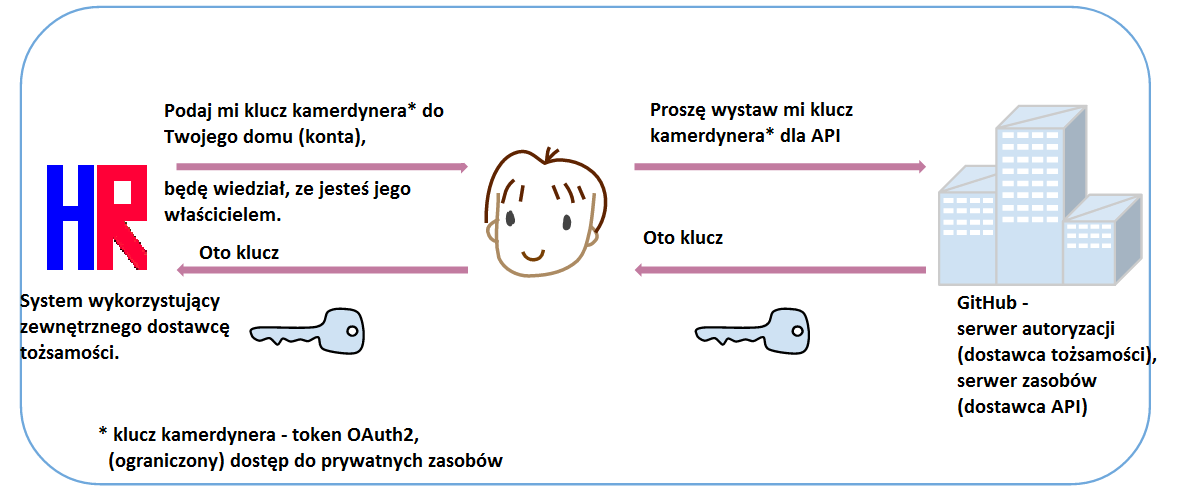
\includegraphics[width=\textwidth]{1_3oauth2}
    \caption[Przebieg uwierzytelnienia z~użyciem protokołu OAuth2]{Przebieg autoryzacji z~użyciem protokołu OAuth2. (Tłumaczenie własne zasobów Wikimedia Commons. Plik udostępniony na licencji Creative Commons CC0 1.0 Uniwersalna Licencja Domeny Publicznej. Pierwotni autorzy: Saqibali, Amada44, Perhelion.)}
    \label{obr13}
\end{figure}


\subsection{System formularzy}

System formularzy autor napisał na nowo, mimo iż istnieje wiele systemów tego typu. Podstawowym wymaganiem w~stosunku do systemu formularzu był dostęp do programistycznego API, który pozwoli założyć, kasować i~odczytywać historię odpowiedzi z~poziomu kodu. Usługa musiała być też darmowa, lub udostępniać darmowy dostęp do celów akademickich. Przetestowano wiele rozwiązań, jednak żadna z~nich nie była satysfakcjonująca dla potrzeb tego projektu. Z~tego autor powodu zdecydował się napisać prosty autorski system formularzy, dopasowany na miarę do realizowanego systemu.

% ex: set tabstop=4 shiftwidth=4 softtabstop=4 noexpandtab fileformat=unix filetype=tex spelllang=pl,en spell:

